\section{Eindimensionale Richtungsbestimmung}
Um den Algorithmus, der aus den Phasendifferenzen die Richtung errechnet, zu entwickeln, haben wir mit der
einfachsten Stufe der Richtungsbestimmung, der eindimensionalen Richtungsbestimmung, angefangen:
\begin{figure}[H]
    \centering
    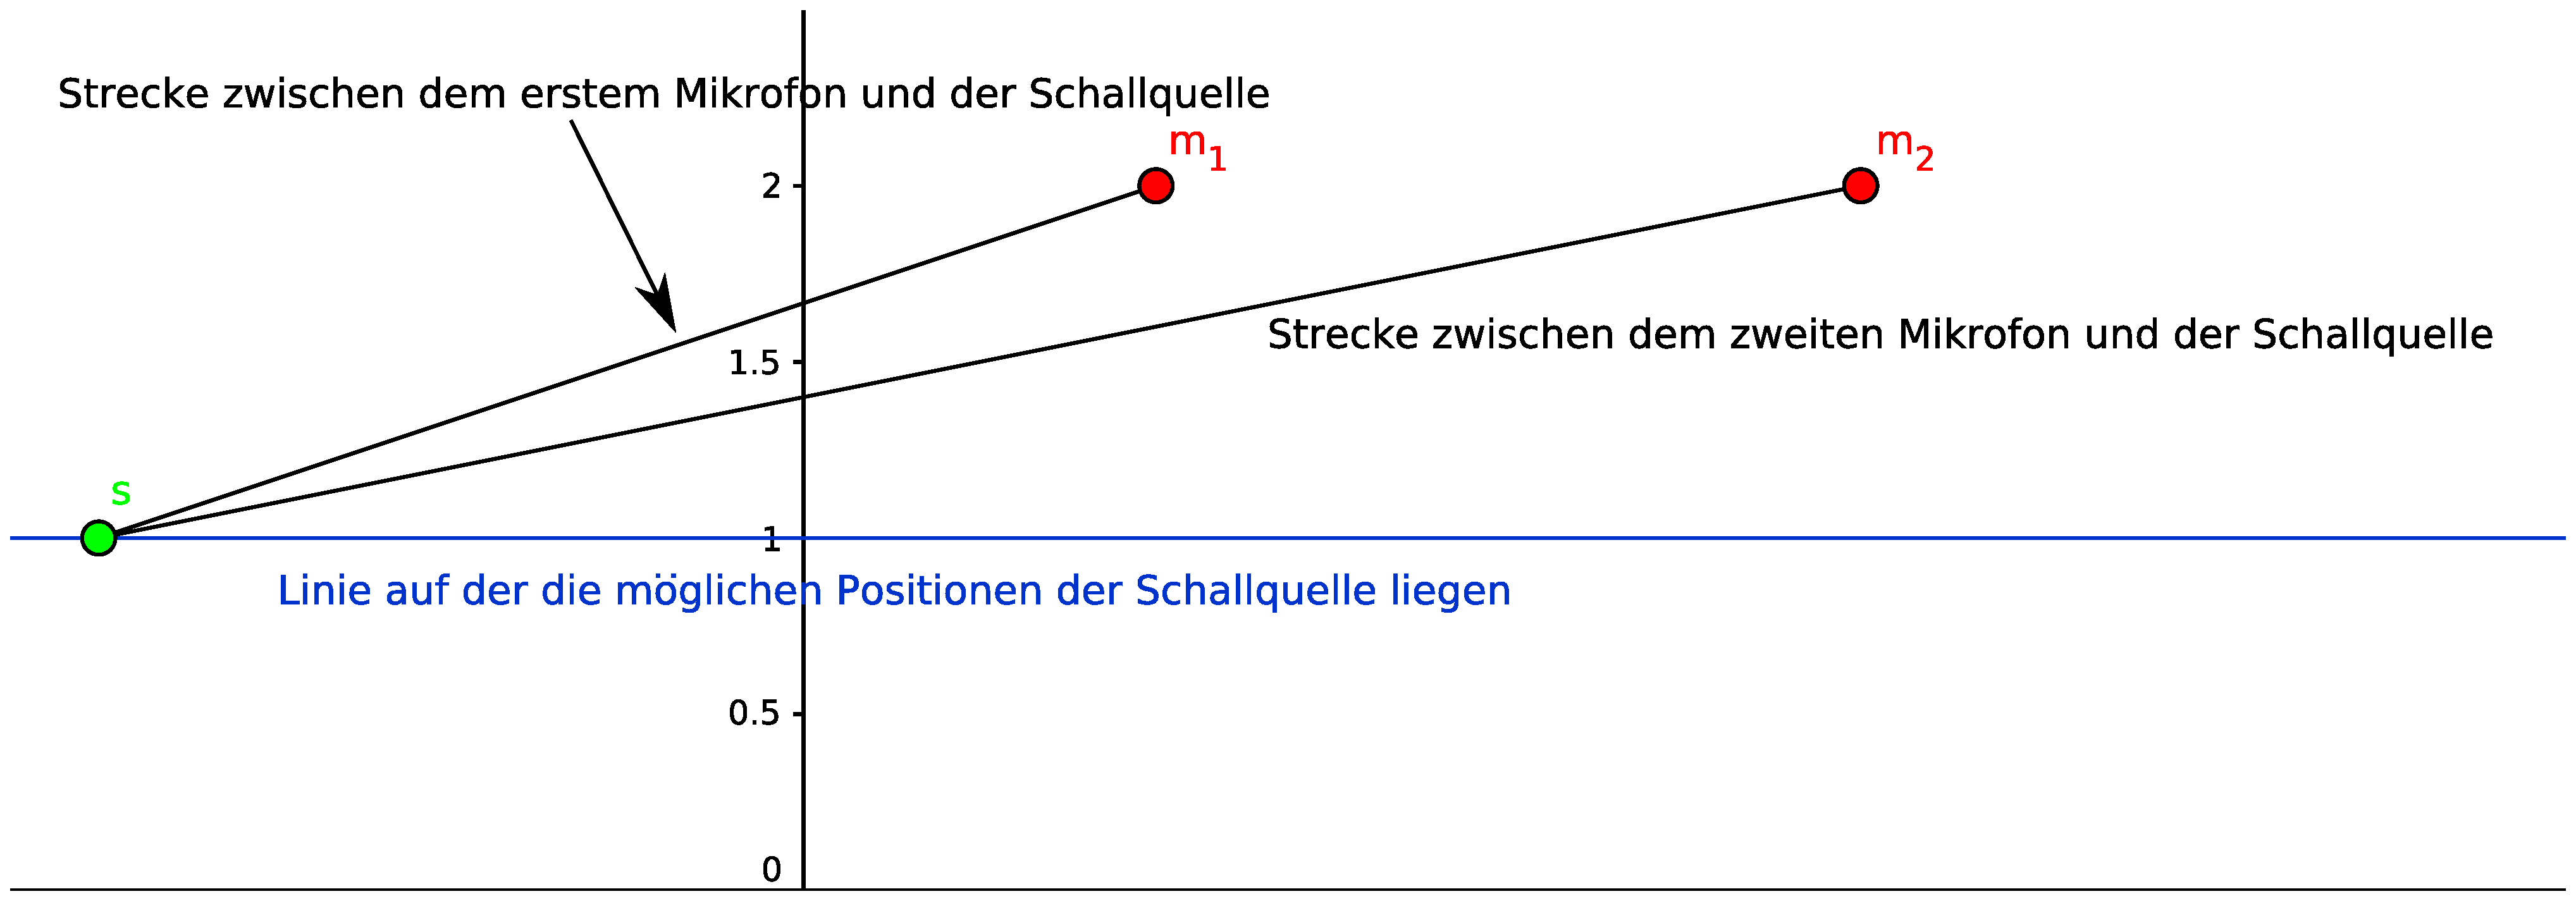
\includegraphics[width=\linewidth]{img/skizze}
    \caption{Skizze einer eindimensionalen Richtungsbestimmung\label{fig:skizz1d}}
\end{figure}

In Abbildung~\ref{fig:skizz1d} sieht man zwei Mikrofone $M_1$ und $M_2$, die den Schall der Schallquelle $S$ aufnehmen. Dadurch, dass $M_2$ weiter von der Schallquelle entfernt ist als $M_1$, braucht der Schall länger, um $M_2$ zu erreichen. Diesen Zeitunterschied sieht man in den von den Mikrofonen aufgenommenen Signalen als Gangunterschied. Man kann von den Wellen, die durch die Mikrofone aufgenommenen werden, nur die Phasenverschiebung bestimmen. Deswegen können wir den Gangunterschied nicht direkt bestimmen, er setzt sich aus einer unbekannten Anzahl von kompletten Schwingungen und der Differenz $d$ der Phasenverschiebungen zusammen. Man erhält für die Differenz der Abstände einer Schallquelle $S$ von zwei Mikrofonen $M_1$ und $M_2$ mit der gemessenen Phase $\phi_1$ und $\phi_2$: $$d = n\lambda + \Delta{x_{12}}$$ $\lambda$ ist hierbei die Wellenlänge, $n$ die unbekannte Anzahl an Schwingungen und $\Delta{x_{12}}$ der Gangunterschied, den man aus dem Phasenunterschied bestimmen kann:
\begin{equation}
\Delta{x_{ij}} = \frac{c(\phi_i - \phi_j)}{{2\pi}f}\:\textrm{mit}\:i = 1\:\textrm{und}\:j = 2
\end{equation}
$c$ ist die Schallgeschwindigkeit und $f$ die Frequenz der Schallwelle.
Jedes Mikrofon $M_i$ hat einen zugehörigen Ortsvektor $\vec{m}_i = \begin{pmatrix} m_{ix} \\ m_{iy}  \end{pmatrix}$, die Schallquelle hat den Ortsvektor $\vec{s} = \begin{pmatrix} {s_x} \\ {s_y}  \end{pmatrix}$. Der Abstand eines Mikrofons von der Schallquelle ist gegeben durch den Satz des Pythagoras:
\begin{equation}
\abs{\vec{m}_i - \vec{s}} = \sqrt{{(m_{ix} - s_x)}^2 + {(m_{iy} - s_y)}^2}
\end{equation}
Damit erhält man für die Differenz der Abstände der Mikrofone die Gleichung
\begin{gather}
\abs{\vec{m}_1 - \vec{s}} - \abs{\vec{m}_2 - \vec{s}} = n\lambda + \Delta{x_{12}}\\
\sqrt{{(m_{1x} - s_x)}^2 + {(m_{1y} - s_y)}^2} - \sqrt{{(m_{2x} - s_x)}^2 + {(m_{2y} - s_y)}^2} = n\lambda + \Delta{x_{12}}
\end{gather}
$s_y$ ist konstant für alle möglichen Positionen der Schallquelle. Dadurch hat die Gleichung aber immer noch zwei Unbekannte, $s_x$ und $n$, und ist deswegen nicht eindeutig lösbar. Man kann eine eindeutig lösbare Gleichung erhalten, wenn der Abstand der Mikrofone maximal halb so groß wie die Wellenlänge ist. Dann macht die Welle maximal eine halbe Schwingung mehr zu einem Mikrofon als zu dem anderen und die unbekannte Anzahl an Schwingungen $n\lambda$ entfällt. Dann hat die Gleichung nur eine Unbekannte, $s_x$.
\begin{gather}
\abs{\vec{m}_1 - \vec{s}} - \abs{\vec{m}_2 - \vec{s}} = \Delta{x_{12}}\\
\sqrt{{(m_{1x} - s_x)}^2 + {(m_{1y} - s_y)}^2} - \sqrt{{(m_{2x} - s_x)}^2 + {(m_{2y} - s_y)}^2} = \Delta{x_{12}}
\end{gather}
Den dadurch bestimmten Ortsvektor kann man dann in einen Strahl $g$ umwandeln, der in die Richtung der Schallquelle weist:
\begin{equation}
g: \vec{x} = \vec{m} + r \cdot (\vec{s} - \vec{m})\quad r \in \mathbb{R}^+
\end{equation}
$\vec{m}$ entspricht dabei der Mitte der Mikrofone und $\vec{x}$ einer beliebigen Position auf der Geraden.\\
Da eine eindimensionale Ortung sehr einfach und ohne großen Anwendungsbereich ist, haben wir diesen Algorithmus anschließend auf zwei Dimensionen übertragen.
